% !TEX root = ../main.tex
% Section 5. Page budget: about 1 page (trimming pass, 2026-11-24).
% Filled by #75 stage 1 (R5). Sources: data/captures/README.md (#68) and data/captures/cap1.pcapng.gz,
% decoded with tshark 4.2.2 and tools/wireshark/meshsync.lua (#87). Every value below was
% read from the capture with tshark (cap1 frame 317 unless stated). MACs in the capture are
% anonymised (scripts/measure/anon_mac.py).
\section{Packet capture and encapsulation analysis (R5)}
\label{sec:capture}

\textbf{Method.} We captured a plain-mode sync of a 100\,MiB file from kratos to defalt with
\code{tshark} on kratos, keeping the first 256 bytes of each frame. Plain mode is our approved R5
deviation, since TLS would hide our messages. MAC addresses were anonymised before commit. Our
Wireshark dissector decodes the meshsync header as its own layer. Figure~\ref{fig:capture} shows one CHUNK\_REQ from defalt.
% tshark -s 256 -f "udp port 47000 or tcp port 47001" on wlp2s0; data/captures/README.md ("How
% they were taken", "Privacy"); tools/wireshark/README.md (D5).
% Figure: Wireshark screenshots by Ahmed (2026-11-25), selected detail lines stacked and
% annotated per layer (layout only; no values changed).

\IfFileExists{figures/capture-chunkreq.png}{%
  \repfigure{capture-chunkreq.png}{One CHUNK\_REQ in Wireshark with our dissector (capture
  \code{cap1}, frame 317), annotated by layer. Selected lines of each header are shown; the red box
  marks our 12-byte header in the packet bytes.}{fig:capture}{0.42\textheight}%
}{%
  \placeholderfigure{Wireshark screenshot of cap1 frame 317, saved as
  report/figures/capture-chunkreq.png}{One CHUNK\_REQ in Wireshark with the meshsync dissector
  (capture \code{cap1}, frame 317), every layer expanded.}{fig:capture}%
}

Each layer adds what the one above lacks: the link header delivers the frame across the Wi-Fi
LAN, IP addresses the other host, TCP reaches our process by port with a reliable, ordered stream,
and our header marks each message's boundary, type and request ID.
% cap1 frame 317: eth.dst/src/type, ip.src/dst/len/ttl/proto/flags.df, tcp.srcport/dstport/seq/
% ack/flags/window_size_value (scale 128)/options, meshsync.* (tshark -V with meshsync.lua).

\textbf{Encapsulation.} Each layer wraps the one above in its own header (Figure~\ref{fig:encap}).
On kratos each header is read by the matching layer and removed: the frame by the network card,
IP and TCP by the kernel, and our header by meshsync. Only the link header changes from hop to hop.

\begin{figure}[H]\centering
  % Encapsulation of one CHUNK_REQ (R5): cap1 frame 317. TikZ fragment, \input by
% report/sections/05-capture.tex. Sizes from tshark: frame.len 154, eth 14, ip.hdr_len 20,
% tcp.hdr_len 32, meshsync header 12, body_len 76 (88 TCP payload, 120 segment, 140 packet).
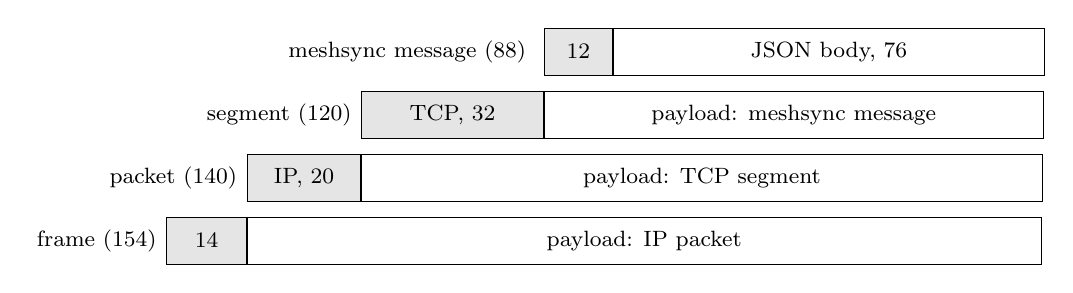
\begin{tikzpicture}[font=\footnotesize, box/.style={draw, minimum height=6mm, inner sep=2pt},
    hd/.style={box, fill=black!10}, pl/.style={box, fill=white}]
  \def\u{0.072} % cm per byte
  % row 4: application message
  \node[hd, minimum width=12*\u cm, anchor=west] (mh) at (6.6,0) {12};
  \node[pl, minimum width=76*\u cm, anchor=west] (mb) at (mh.east) {JSON body, 76};
  \node[anchor=east] at (6.5,0) {meshsync message (88)};
  % row 3: TCP segment
  \node[hd, minimum width=32*\u cm, anchor=east] (th) at (6.6,-0.8) {TCP, 32};
  \node[pl, minimum width=88*\u cm, anchor=west] (tp) at (th.east) {payload: meshsync message};
  \node[anchor=east] at (th.west) {segment (120)};
  % row 2: IP packet
  \node[hd, minimum width=20*\u cm, anchor=east] (ih) at (th.west |- 0,-1.6) {IP, 20};
  \node[pl, minimum width=120*\u cm, anchor=west] (ip) at (ih.east) {payload: TCP segment};
  \node[anchor=east] at (ih.west) {packet (140)};
  % row 1: frame
  \node[hd, minimum width=14*\u cm, anchor=east] (fh) at (ih.west |- 0,-2.4) {14};
  \node[pl, minimum width=140*\u cm, anchor=west] (fp) at (fh.east) {payload: IP packet};
  \node[anchor=east] at (fh.west) {frame (154)};
\end{tikzpicture}

  \caption{Encapsulation of the CHUNK\_REQ in frame 317, in bytes. Grey: each layer's header.}
  \label{fig:encap}
\end{figure}
% Sizes: frame.len 154, ip.len 140, tcp.hdr_len 32, tcp.len 88, meshsync.body_len 76.

\textbf{Overhead.} In this small frame 78 of 154 bytes are headers, only 12 of them ours. Over the
whole 100\,MiB transfer our messages added 0.21\,\% and all headers 5.98\,\%.
% cap1 frame 225: frame.len 1514, tcp.len 1448, CHUNK_DATA body_len 65558. Whole transfer:
% data/captures/README.md ("Header and body overhead").
